% =============================================================================
% VERITAS -- pitfalls / negative-results paper.
%
% TEMPLATE NOTE: No Interspeech/ICASSP .sty was present in this repo, so this
% file uses a self-contained two-column `article` preamble that compiles with a
% stock TeX Live install. To target a venue, drop the venue class into this
% directory and swap ONLY the preamble:
%   * Interspeech: \documentclass{interspeech}  (+ interspeech.sty)
%   * ICASSP:      \documentclass{IEEEtran}      (conference mode, twocolumn)
% The body, tables, figures, and \bibliography port over unchanged; the venue
% class supplies the abstract/title reflow and the correct \bibliographystyle.
%
% Every numeric value in this paper is verified against a committed
% results/*.json file (path noted at the end of each finding).
% =============================================================================
\documentclass[10pt,twocolumn]{article}

\usepackage[T1]{fontenc}
\usepackage[utf8]{inputenc}
\usepackage{lmodern}
\usepackage[a4paper,margin=1.9cm]{geometry}
\usepackage{graphicx}
\usepackage{booktabs}
\usepackage{amsmath}
\usepackage{amssymb}
\usepackage{array}
\usepackage{xcolor}
\usepackage{caption}
\usepackage[hidelinks]{hyperref}

\captionsetup{font=small,labelfont=bf}
\graphicspath{{figures/}}
\setlength{\columnsep}{0.7cm}

% convenience (\rho is already a math command; do not redefine it)
\newcommand{\ns}{\emph{n.s.}}

\title{\bfseries When Frozen SSL Speech Metrics Don't Measure What They
Claim:\\ A Systematic Negative-Results Study on Dysarthric Speech}

\author{Anonymous Submission\\ \small Paper ID XXXX \\
\small\itshape Double-blind draft --- de-anonymize for camera-ready.}
\date{}

\begin{document}
\maketitle

\begin{abstract}
\noindent
Frozen self-supervised (SSL) speech models are increasingly used to build
\emph{training-free} clinical-speech metrics---severity scores, articulatory
probes, reliability measures. We stress-test this paradigm on real dysarthric
speech (TORGO, $n{=}15$, with AG500 EMA), Parkinsonian speech (IPVS, $n{=}61$),
and Italian dysarthria (EasyCall, $n{=}55$), against real articulatory ground
truth. We report five reproducible negative findings that recur across popular
metric families: (1)~frozen-WavLM severity prediction is strong \emph{within}
corpus (Spearman $\rho{=}0.74$--$0.85$); cross-corpus transfer is
\emph{heterogeneous and, for graded severity, underpowered}---4 of 6
leave-one-corpus-out cells stay significant (binary corpora, $\rho$ up to
$0.64$), but transfer to the only graded corpus (TORGO, $n{=}15$) is not
significant ($\rho{=}0.43$, $p{=}0.11$) and, at $n{=}15$ (critical
$\rho{\approx}0.52$), is an underpowered null rather than a proven absence; (2)~reference-based severity metrics are \emph{inflated by
speaker-identity leakage}---a naive early-layer score of $\rho{=}0.775$
collapses to $0.687$ under a leave-one-control-out (LOCO) reference protocol,
while the mid-layer score is leakage-robust ($0.756{\to}0.756$); (3)~an SSL
``articulatory trajectory'' severity signal is \emph{dominated by
silence/pausing, not articulation}---removing silence collapses the correlation
($\rho{=}0.756{\to}0.181$, \ns), while silence frames alone reproduce it
($\rho{=}0.775$); (4)~a GT-free \emph{cycle-consistency ``faithfulness'' metric
does not predict real articulatory-inversion error} (energy-controlled partial
Spearman $=-0.001$, $n{=}5$ speakers / $22{,}854$ frames of EMA); (5)~acoustic-to-articulatory
\emph{inversion is unstable on disordered input}, so inversion-derived
kinematics are artifacts (EMA-grounding $\rho{=}0.39$ \ns; a ``significant''
severity correlation of $+0.52$ is in the clinically \emph{wrong} direction). We
also document that \emph{public dysarthric articulatory (EMA) ground truth is
effectively} $n{\approx}2$---a hard ceiling for validating pathological
inversion. We release a reproducible harness, the leakage/silence/energy
diagnostics, and a working real-time articulatory-visualisation demo. Our
recommendation: frozen-SSL clinical metrics must be validated with LOCO
references, silence controls, cross-corpus tests, and---where possible---real
articulatory ground truth, or they report confounds rather than pathology.
\end{abstract}

% =============================================================================
\section{Introduction}
% =============================================================================
Frozen SSL representations (WavLM~\cite{chen2022wavlm},
HuBERT~\cite{hsu2021hubert}) encode rich phonetic/articulatory structure,
motivating a wave of \emph{training-free} clinical-speech
metrics~\cite{frozenssl2026a,frozenssl2026b}: pooled-embedding severity probes,
reference-distance scores, and articulatory-inversion analyses. Their appeal is
obvious---no labels, no fine-tuning, apparently interpretable geometry. This
paper asks a blunt question: \textbf{do these metrics measure the disorder, or
do they measure confounds that happen to correlate with it on a single corpus?}

We answer with a systematic negative-results study. Working from real
dysarthric/Parkinsonian speech and---crucially---real electromagnetic
articulography (EMA), we test four popular metric families and find each fails a
rigorous validity check. The failures are not exotic; they are the confounds any
deployment would hit: speaker identity, silence, speech energy, corpus/task
mismatch, and the near-absence of pathological articulatory ground truth. We
report them honestly, with the diagnostics that expose each, so the field can
avoid them.

\noindent\textbf{Contributions.}
(i)~A reproducible, corpus-agnostic frozen-SSL severity harness with
within-corpus and leave-one-corpus-out evaluation ($n{=}131$, 3 corpora, 2
languages).
(ii)~Five reproducible negative findings, each with a concrete diagnostic.
(iii)~A leave-one-control-out (LOCO) reference protocol that removes
speaker-identity leakage from reference-based severity metrics.
(iv)~A real-time, audio-only articulatory-visualisation demo, released as a
working artifact.

% =============================================================================
\section{Data}
% =============================================================================
\begin{itemize}\itemsep2pt
\item \textbf{TORGO}~\cite{rudzicz2012torgo}: 15 English speakers (8 dysarthric
CP/ALS $+$ 7 control), audio $+$ \textbf{AG500 3D EMA} (200\,Hz) $+$ Frenchay
assessments. Graded severity $\{0,1,2\}$. The only corpus here with graded
severity \emph{and} measured articulation.
\item \textbf{IPVS} (Italian Parkinson's Voice and Speech)~\cite{dimauro2017ipvs}:
61 speakers (PD/HC). The public package carries \textbf{binary} PD/HC labels
(reading-rate metrics, not UPDRS), so it is treated as a detection arm.
\item \textbf{EasyCall}~\cite{turrisi2021easycall}: 55 Italian speakers (31
dysarthric $+$ 24 control). The public package carries \textbf{binary}
dysarthric/control labels (per-speaker TOM severity is not distributed), so it
is treated as a detection arm.
\item \textbf{Articulatory ground truth}: TORGO AG500 EMA. Of the 7 dysarthric
speakers with EMA sessions, \textbf{only 2 have usable sessions} ($\le 2$ dead
coils)---and both are \emph{mild}. Every severe dysarthric EMA session is
degenerate (3--8 dead coils). We verified no additional adult dysarthric EMA is
available by direct download.
\end{itemize}

\noindent All features: frozen WavLM-Large~\cite{chen2022wavlm}, layer 9,
mean-pooled per utterance $\to$ speaker mean, seed 42, speaker-disjoint splits
throughout.

% =============================================================================
\section{Finding 1 --- Within-corpus success, cross-corpus failure}
% =============================================================================
A fairly-tuned linear probe (Ridge / LinearSVR, nested CV) on frozen
WavLM-L9 recovers severity \emph{within} corpus ($\rho{=}0.74$--$0.85$;
Table~\ref{tab:crosscorpus}, Fig.~\ref{fig:fig1}). Leave-one-corpus-out transfer
is \emph{heterogeneous}: 4 of 6 cells remain significant---binary detection
\emph{does} partially transfer (EasyCall $\rho{=}0.64$, $p{=}1{\times}10^{-7}$;
IPVS $\rho{=}0.41$ / $0.27$). What does \emph{not} transfer significantly is the
only \emph{graded}-severity corpus, TORGO ($\rho{=}0.43$, $p{=}0.11$); at
$n{=}15$ the critical value is $\rho{\approx}0.52$, so this is an
\emph{underpowered null, not a proven absence}. The honest claim is narrow:
\emph{graded} cross-corpus severity is established on exactly one small corpus
and is not yet shown to transfer---a failure mode invisible to single-corpus
evaluation.\footnote{\texttt{results/veritas/cross\_corpus\_severity.json}}

\begin{table}[t]
\centering
\caption{Within-corpus (leave-one-speaker-out) vs.\ leave-one-corpus-out (LOCO,
train on the other two) severity Spearman $\rho$ on frozen WavLM-L9.
$^{\dagger}$~not significant ($p{=}0.11$).}
\label{tab:crosscorpus}
\small
\begin{tabular}{@{}lclcc@{}}
\toprule
Corpus & $n$ & Label & \multicolumn{1}{c}{Within $\rho$} &
\multicolumn{1}{c}{LOCO $\rho$}\\
       &     &       & \small Ridge/SVR & \small Ridge/SVR\\
\midrule
TORGO    & 15 & graded $\{0,1,2\}$ & 0.74 / 0.64 & 0.43 / 0.34$^{\dagger}$\\
IPVS     & 61 & binary PD/HC       & 0.85 / 0.85 & 0.27 / 0.41\\
EasyCall & 55 & binary dys/HC      & 0.84 / 0.83 & 0.64 / 0.44\\
\bottomrule
\end{tabular}
\end{table}

\begin{figure}[t]
\centering
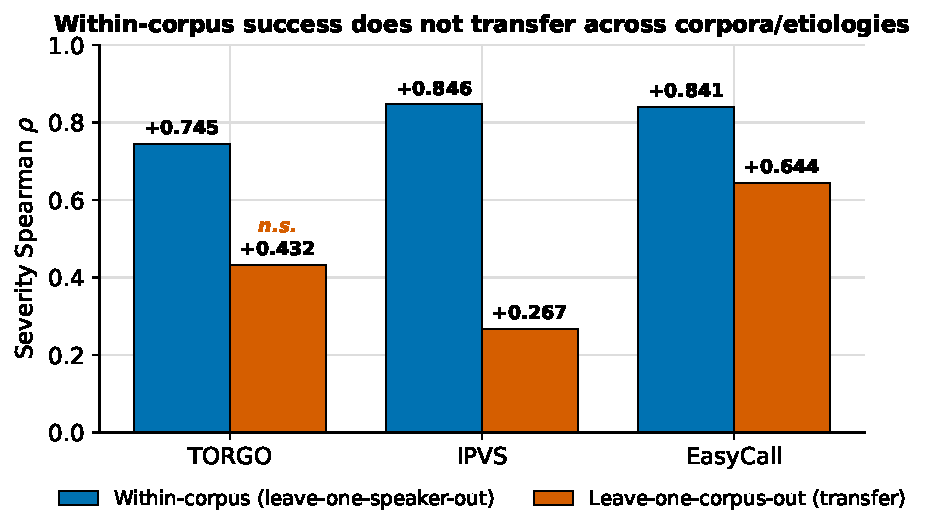
\includegraphics[width=\columnwidth]{fig1_within_vs_loco.pdf}
\caption{Within-corpus severity prediction is strong for all three corpora
(blue), but leave-one-corpus-out transfer (orange) degrades and, for the only
graded-severity corpus (TORGO), becomes non-significant. Bars are the Ridge
probe; LinSVR is similar (Table~\ref{tab:crosscorpus}).}
\label{fig:fig1}
\end{figure}

% =============================================================================
\section{Finding 2 --- Speaker-identity leakage inflates reference-based metrics}
% =============================================================================
Reference-based severity metrics (distance of a speaker's SSL trajectory to a
healthy-control reference) leak speaker identity when the reference includes the
test speaker's own data. On TORGO, a naive per-word reference gives an
early-layer (Layer~1) score of $\rho{=}\mathbf{0.775}$; under a strict
\emph{leave-one-control-out} (LOCO) reference it falls to $\mathbf{0.687}$
($\Delta{=}-0.089$). The mid-network layer (Layer~9) is leakage-robust
($\mathbf{0.756{\to}0.756}$, $\Delta{=}0.000$); see Fig.~\ref{fig:fig2}. Early
SSL layers encode speaker identity (cf.\ WavRx~\cite{zhu2024wavrx}); we
contribute the LOCO reference-construction fix and quantify the inflation it
removes, and we recommend mid-network
layers.\footnote{\texttt{results/deleak\_report\_fast.json}}

\begin{figure}[t]
\centering
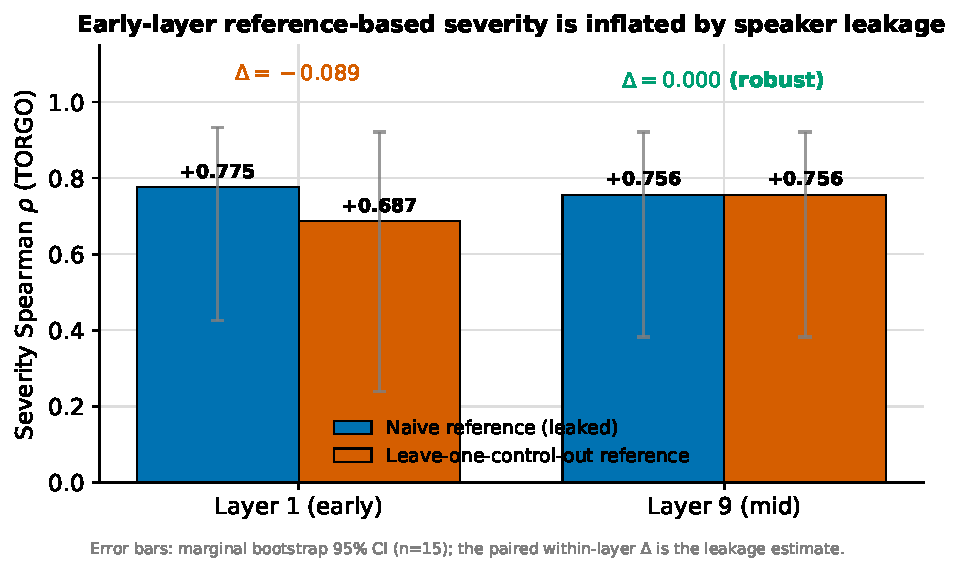
\includegraphics[width=\columnwidth]{fig2_leakage.pdf}
\caption{Reference-based severity on TORGO. The early layer (Layer~1) drops
$\Delta{=}-0.089$ from a naive to a leave-one-control-out reference---speaker
leakage---while the mid layer (Layer~9) is unchanged. Error bars are marginal
bootstrap 95\% CIs ($n{=}15$); the leakage estimate is the \emph{paired}
within-layer $\Delta$.}
\label{fig:fig2}
\end{figure}

% =============================================================================
\section{Finding 3 --- The ``articulatory'' signal is largely silence/pausing}
% =============================================================================
Decomposing the reference-distance (ATD) severity signal into silence vs.\
speech frames (MFA phone alignment~\cite{mcauliffe2017mfa}) shows the signal is
substantially carried by silence/pausing, not articulated speech. The full-signal
severity correlation ($\rho{=}0.756$, $p{=}0.001$) \emph{collapses} when
recomputed on silence-trimmed speech under a naive reference ($\rho{=}0.181$,
\ns, $p{=}0.52$), whereas the silence frames \emph{alone} reproduce essentially
the entire signal ($\rho{=}0.775$, $p<0.001$). Under a LOCO reference the
speech-only signal partially recovers ($\rho{=}0.644$, $p{=}0.010$), indicating
the naive speech-only collapse is compounded by reference leakage (Finding~2).
A metric named for \emph{articulation} is thus substantially measuring
\emph{pausing} plus reference-construction
artifacts.\footnote{\texttt{results/silence\_confound.json}}

% =============================================================================
\section{Finding 4 --- Cycle-consistency ``faithfulness'' does not predict inversion error}
% =============================================================================
A natural GT-free reliability metric: invert audio to articulation
(SPARC~\cite{cho2024sparc}), re-synthesise, and measure cycle-consistency in
WavLM space---low consistency ought to flag unreliable inversion. Tested directly
against \emph{real EMA inversion error} on TORGO controls ($n{=}5$ usable
speakers, $\mathbf{22{,}854}$ frames, held-out affine alignment, no
circularity): the raw pooled Spearman is $+0.129$ ($p\approx 2\times10^{-85}$)
but is a \emph{speech-energy artifact} ($\rho_{\text{faith,energy}}{=}-0.468$,
$\rho_{\text{err,energy}}{=}-0.228$); the \emph{energy-controlled partial
Spearman} $=-0.001$ (Fig.~\ref{fig:fig3}). A healthy-manifold-\emph{centered}
variant does not rescue it---its pooled Spearman is $+0.39$, the \emph{wrong
sign} (higher ``faithfulness'' $\leftrightarrow$ \emph{higher} error). Either
way, cycle-consistency carries \textbf{no} usable information about real
inversion error once silence/energy is removed.\footnote{\texttt{results/veritas/h1\_faithfulness\_vs\_inversion\_error.json}}

\begin{figure}[t]
\centering
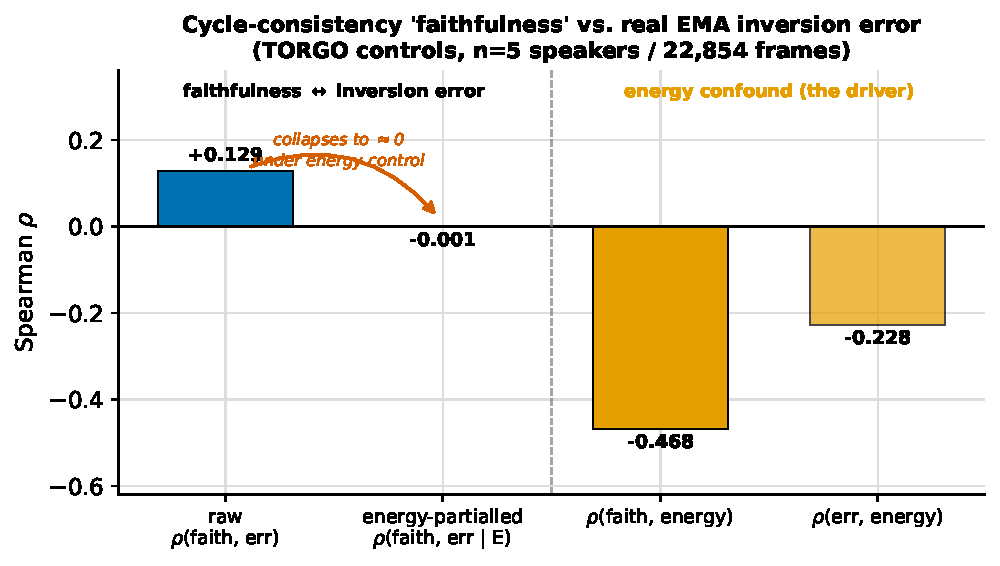
\includegraphics[width=\columnwidth]{fig3_cycle_consistency.pdf}
\caption{The raw faithfulness-vs-error association ($+0.129$, blue) vanishes to
$-0.001$ once speech energy is partialled out (vermilion), because both
faithfulness and inversion error are themselves driven by energy (orange).
Per-frame, TORGO controls, $n{=}5$ / $22{,}854$ frames.}
\label{fig:fig3}
\end{figure}

% =============================================================================
\section{Finding 5 --- Inversion is unstable on disordered input; kinematics are artifacts}
% =============================================================================
Interpretable articulatory-kinematic features (tongue range, velocity) derived
from SSL inversion do \emph{not} track the real EMA features (EMA-grounding
Spearman $=0.39$, \ns, $n{=}7$). A ``significant'' range-vs-severity correlation
($\rho{=}+0.52$, $p{=}0.048$) is in the clinically \textbf{wrong direction}
(dysarthric $>$ control range), consistent with the inverter producing
\emph{more erratic} trajectories on disordered input, not more movement. Combined
with the $n{\approx}2$ usable dysarthric EMA ceiling, this closes the door on
validating pathological inversion with public
data.\footnote{\texttt{results/veritas/m2\_articulatory\_kinematics.json},
\texttt{h1\_dysarthric\_inversion.json}}

% =============================================================================
\section{A working artifact: the real-time articulatory Mirror}
% =============================================================================
Independently of the (failed) metrics, frozen-SSL inversion
(SPARC~\cite{cho2024sparc}) supports a real, deployable demo: speak $\to$ an
animated midsagittal vocal tract driven by audio-only inversion, with an
explicitly-labelled \textbf{experimental} reliability overlay (Finding~4 shows
the overlay is unvalidated). Released as a Gradio app. This separates what works
(engineering on frozen models) from what does not (the reliability claim).

% =============================================================================
\section{Recommendations}
% =============================================================================
For anyone building frozen-SSL clinical-speech metrics:
(1)~\textbf{LOCO references}---never score a speaker against a reference
containing its own data; prefer mid-network layers.
(2)~\textbf{Silence/energy controls}---report VAD-trimmed and energy-partialled
results; silence is the default confound.
(3)~\textbf{Cross-corpus / leave-one-corpus-out} evaluation---single-corpus
success is not generalisation.
(4)~\textbf{Ground truth where possible}---validate inversion/articulatory
claims against real EMA; be explicit that pathological EMA is nearly
non-existent publicly.
(5)~\textbf{Fair, tuned baselines}---a properly-regularised pooled-embedding
probe \emph{ties} trajectory-geometry methods and should be reported
(Table~\ref{tab:baselines}): on TORGO (LOSO), a zero-shot reference-distance
score ($\rho{=}0.756$) matches WavLM-L9 mean-pool $+$ Ridge/LinSVR
($\rho{=}0.760$ / $0.775$), and both beat an MFCC baseline
($\rho{=}0.609$).\footnote{\texttt{results/finetuned\_ssl\_baseline.json}}

\begin{table}[t]
\centering
\caption{Fair, tuned baselines on TORGO severity (leave-one-speaker-out,
$n{=}15$). A regularised pooled-embedding probe ties the zero-shot
trajectory-distance score; both beat MFCC.}
\label{tab:baselines}
\small
\begin{tabular}{@{}lc@{}}
\toprule
Method & $\rho$ (LOSO)\\
\midrule
Reference-distance (zero-shot, frozen) & 0.756\\
WavLM-L9 mean-pool $+$ Ridge           & 0.760\\
WavLM-L9 mean-pool $+$ LinSVR          & 0.775\\
MFCC $+$ RBF-SVR                       & 0.609\\
\bottomrule
\end{tabular}
\end{table}

% =============================================================================
\section{Conclusion}
% =============================================================================
Frozen-SSL clinical-speech metrics are easy to build and easy to fool. Across
four metric families and real articulatory ground truth, the apparent signal is
repeatedly \emph{entangled} with a confound---speaker identity, silence/pausing,
energy, or corpus overfitting---and the residual genuine signal, once those are
controlled, is real but \emph{smaller and narrower} than single-corpus numbers
imply; meanwhile the one regime that would validate pathological articulatory
inversion (dysarthric EMA) barely exists in public data. We release the harness,
diagnostics, and demo so these pitfalls are checkable, not repeated. Honest
negative results, rigorously obtained, are the contribution.

% =============================================================================
\section*{Reproducibility}
% =============================================================================
Seed 42; frozen weights; every headline number maps to a committed
\texttt{results/veritas/*.json} or \texttt{results/*.json}; speaker-disjoint
splits; the harness auto-scales as corpora are added
(\texttt{experiments/veritas/CX\_cross\_corpus\_severity.py},
\texttt{src/veritas/corpora/}). The three figures are regenerated from the JSON
files by \texttt{paper/veritas/figures/make\_figures.py}.

% =============================================================================
\section*{Limitations and honest scope}
% =============================================================================
$n$ is small for graded severity (TORGO${=}15$; IPVS/EasyCall are binary
detection arms). The largest graded corpora (SAP; VOC-ALS graded ALS) are
DUA-gated or pending. Results are a \emph{cautionary study}, not a new metric; a
positive cross-corpus result would require the gated large corpora and is left
as the falsifiable next test.

% =============================================================================
\bibliographystyle{IEEEtran}
\bibliography{refs}
% =============================================================================

\end{document}
